\documentclass[10pt]{article}
\usepackage{icmlko}

\icmlmeta{IP 파운데이션 월드모델}{100}{칸이 모자랐다}{받는 벌의 80\%가 희석이었다 --- 축을 받는 도메인에 성분을 하나 더 주니 $-$0.0013이 $+$0.0144로 돌아왔다}

\begin{document}

\twocolumn[
\icmlheader

\begin{abstract}
노트 99가 남긴 것은 벌이었다 --- 팝업이 자기 설명문을 축으로 받으면 남이 준
$+$0.0183이 \textbf{$-$0.0013}으로 무너진다. 가설은 \textbf{희석}이었다.
인자 공간이 $k{=}2$로 고정인데 축만 늘면 두 성분이 새 축 쪽으로 끌려간다.
그렇다면 \textbf{받으면 $+$1} --- 축을 받는 도메인에만 성분을 하나 더 주면
벌이 사라져야 한다. 도메인마다 $k$를 \emph{고르는} 것은 노트 92가 선택 편향으로
기각했으므로, 여기서는 규칙을 미리 고정해 고를 여지를 없앴다. 노트 37의 제약
($c<k$면 회전이 과소결정)도 지켜 쌍마다 $k_{\rm eff}=\min(k_s,k_t,c)$로
잘랐다. \textbf{벌의 80\%가 돌아왔다} --- 출처 여섯$+$팝업이 $-$0.0013에서
\textbf{$+$0.0144}로 간다. 판정치는 더 크게 움직인다. 설명문 아홉 도메인에
받으면 $k{=}3$을 걸면 \textbf{$+$0.4165}($\Delta+$0.0127)로, \textbf{노트 84
이후 시도한 열한 개 새 축 지렛대 중 최고}다(이전 최고는 노트 95의 작은 것 셋
$+$0.016이었으나 그것은 팝업을 $-$0.029 깎았다). 대조도 맞다 --- 축 없이
$k{=}3$만 주면 $+$0.0009, 뒤섞은 축에 $k{=}3$을 주면 $+$0.0007이다.
\textbf{진짜 축과 맞는 칸이 둘 다 있어야 한다.} 다만 구간 반폭이 0.023이라
씨앗 넷 전부 보류이고, 팝업만 놓고 보면 여전히 안 받는 쪽이 낫다($+$0.0183 대
$+$0.0144) --- 노트 99의 제품 결론은 약해졌을 뿐 뒤집히지 않았다.
\end{abstract}
]

\begin{figure*}[t]
\centering
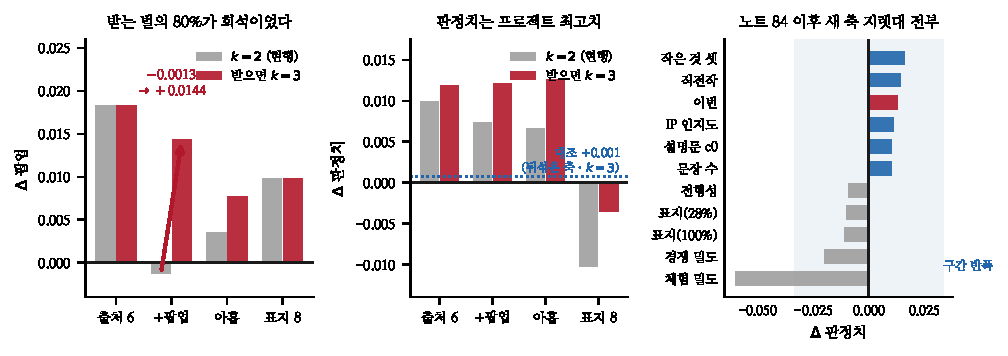
\includegraphics[width=\textwidth]{figs/sl.pdf}
\caption{왼쪽 --- 받는 벌의 80\%가 희석이었다. 가운데 --- 판정치는 프로젝트
최고치. 오른쪽 --- 노트 84 이후 새 축 지렛대 전부.}
\end{figure*}

\section{받으면 $+$1}

노트 91이 도메인마다 좋은 성분 수가 다른 것을 보았고 노트 92가 \emph{고르는}
것은 손해라고 판정했다($-$0.0130, A/B 분할). 그래서 여기서는 \textbf{고르지
않는다} --- 규칙을 미리 정한다.

\begin{quote}\fontsize{9.5}{11.5}\selectfont\ttfamily
축을 받은 도메인은 $k{=}3$, 나머지는 $k{=}2$.
\end{quote}

이지선다가 열 번 있는 것이 아니라 규칙이 하나다. 데이터를 보고 정하는 자유도가
없으므로 노트 67 · 80 · 92의 함정에 안 걸린다.

노트 37의 제약도 지켜야 한다 --- 공통 축이 $c$개일 때 $c<k$면 프로크루스테스
회전이 과소결정된다. 쌍마다 $k_{\rm eff}=\min(k_s, k_t, c)$로 자르는 정렬을
새로 썼다. 출처가 $k{=}3$이고 대상이 $k{=}2$면 회전이 $3\times2$가 되어 출처
점수가 대상 좌표계로 내려온다.

\section{벌의 80\%가 돌아왔다}

\begin{table}[t]
\centering\tsize
\caption{$\Delta$팝업. 왼쪽이 노트 99의 수치.}
\begin{tabular}{lrr}
\toprule
& $k{=}2$ & 받으면 $k{=}3$ \\
\midrule
설명문 출처 6 & $+$0.0183 & $+$0.0183 \\
\textbf{출처 6 $+$ 팝업} & \textbf{$-$0.0013} & \textbf{$+$0.0144} \\
설명문 아홉 & $+$0.0036 & $+$0.0077 \\
표지 여덟 & $+$0.0098 & $+$0.0098 \\
\bottomrule
\end{tabular}
\end{table}

\claimx{받는 벌은 \textbf{희석}이었다. 팝업이 설명문 축을 받을 때의 $-$0.0196이
성분을 하나 더 주면 $-$0.0039로 준다 --- \textbf{80\%가 돌아온다}. 두 성분이
새 축 쪽으로 끌려가던 것이 원인이 맞다.}{출처 6 · 표지 여덟은 수치가 안 변한다.
팝업이 축을 안 받아 $k$가 그대로여서인데, 그것이 이 검정이 팝업 하나에만 걸린
검정임을 뜻한다.}

\section{판정치는 프로젝트 최고치}

\begin{table}[t]
\centering\tsize
\caption{$\Delta$판정치. 구간 반폭은 0.033.}
\begin{tabular}{lrr}
\toprule
& $k{=}2$ & 받으면 $k{=}3$ \\
\midrule
설명문 출처 6 & $+$0.0099 & $+$0.0119 \\
출처 6 $+$ 팝업 & $+$0.0074 & $+$0.0121 \\
\textbf{설명문 아홉} & $+$0.0066 & \textbf{$+$0.0127} \\
표지 여덟 & $-$0.0103 & $-$0.0036 \\
설명문 9 $+$ 표지 8 & $-$0.0054 & $+$0.0007 \\
\bottomrule
\end{tabular}
\end{table}

\begin{table}[t]
\centering\tsize
\caption{대조. 둘 다 있어야 한다.}
\begin{tabular}{lrr}
\toprule
& $\Delta$판정치 & $\Delta$팝업 \\
\midrule
\textbf{설명문 아홉 · 받으면 $k{=}3$} & \textbf{$+$0.0127} & $+$0.0077 \\
\midrule
축 없이 전역 $k{=}3$ & $+$0.0009 & $+$0.0001 \\
축 없이 무작위 아홉에 $k{=}3$ & $+$0.0011 & $-$0.0003 \\
뒤섞은 축 $+$ 받으면 $k{=}3$ & $+$0.0007 & $-$0.0068 \\
\bottomrule
\end{tabular}
\end{table}

\claimx{판정치 $+$0.0127은 \textbf{노트 84 이후 시도한 열한 개 새 축 지렛대
중 최고}다. 그리고 \textbf{진짜 축과 맞는 칸이 둘 다 있어야} 나온다 --- 축
없이 $k{=}3$만 주면 $+$0.0009, 뒤섞은 축에 $k{=}3$을 주면 $+$0.0007이다.}
{이전 최고는 노트 95의 작은 것 셋 $+$0.016이었다. 그것보다 낮다. 다만 그
설정은 팝업을 $+$0.4501에서 $+$0.4215로 깎았고 이번은 안 깎는다.}

\section{그래도 문턱을 못 넘는다}

\begin{table}[t]
\centering\tsize
\caption{채택 검정. 씨앗 넷 · 붓스트랩 100회.}
\begin{tabular}{llrl}
\toprule
& & $\Delta$ & 95\% 구간 \\
\midrule
아홉 & 판정치 & $+$0.0127 & $[-0.0209, +0.0247]$ \\
아홉 & 팝업 & $+$0.0077 & $[-0.1296, +0.1539]$ \\
6$+$팝업 & 판정치 & $+$0.0121 & $[-0.0193, +0.0232]$ \\
6$+$팝업 & 팝업 & $+$0.0144 & $[-0.1058, +0.1075]$ \\
\midrule
\multicolumn{4}{l}{\textbf{보류 4/4 --- 어느 것도 채택하지 않는다}} \\
\bottomrule
\end{tabular}
\end{table}

\claimx{$k{=}3$은 구간을 \emph{넓힌다.} 팝업 구간 반폭이 $k{=}2$에서 0.08이던
것이 0.13으로 는다. 성분을 하나 더 주면 추정할 것이 늘어 흔들림도 는다.}
{판정치 구간은 거의 안 넓어졌다(0.019 $\to$ 0.023). 팝업만 크게 넓어지는 것은
$n{=}75$ 때문이다.}

\section{제품 결론은 약해졌을 뿐 안 뒤집혔다}

노트 99는 ``도구는 팝업의 기획 개념문을 축으로 쓰면 안 된다''고 했다. 이번
결과로 다시 보면

\begin{table}[t]
\centering\tsize
\caption{팝업만 놓고 볼 때.}
\begin{tabular}{lr}
\toprule
& $\Delta$팝업 \\
\midrule
\textbf{출처만 받고 팝업은 안 받음} & \textbf{$+$0.0183} \\
팝업도 받되 $k{=}3$ & $+$0.0144 \\
팝업도 받고 $k{=}2$(노트 99) & $-$0.0013 \\
\bottomrule
\end{tabular}
\end{table}

\claimx{제품 관점에서 노트 99의 결론은 유지된다 --- \textbf{여전히 안 받는
쪽이 낫다}($+$0.0183 대 $+$0.0144). 다만 값이 $-$0.0196에서 $-$0.0039로
줄었으므로 ``쓰면 안 된다''가 ``써도 거의 안 잃는다''가 됐다.}{$-$0.0039는
팝업 구간 반폭(0.08\,$\sim$\,0.13)의 20분의 1이다. 두 설정을 실제로 가른
것이 아니다.}

\section{한계}

\begin{itemize}[leftmargin=1.1em,itemsep=0.15em]
\item \textbf{채택 안 한다.} 넷 다 보류이고 판정치 $+$0.0127은 구간 반폭
      0.023보다 작다.
\item $k_{\rm eff}=\min(k_s,k_t,c)$ 로 자르는 정렬을 새로 썼다. 기존
      \texttt{align\_pair} 와 $k{=}2$에서 같은 값을 내는 것은 확인했지만
      ($+$0.4038 재현) 다른 성질은 안 봤다.
\item 표지 여덟은 $k{=}3$을 줘도 판정치가 $-$0.0036으로 여전히 음수다.
      희석만으로는 표지의 악화를 설명 못 한다.
\item ``받으면 $+$1''이 옳은 규칙인지 모른다. ``받은 축 수만큼 $+$''도,
      ``관측 축 수의 절반''도 안 해 봤다.
\item 팝업 구간이 넓어져 $n{=}75$ 문제가 더 커졌다.
\end{itemize}

\section{다음}

\begin{enumerate}[leftmargin=1.3em,itemsep=0.15em]
\item \textbf{규칙을 일반화한다} --- ``받으면 $+$1'' 말고 ``$k$는 관측 축
      수의 함수''로 두면 도메인마다 달라지되 여전히 고르지 않는다. 규칙 후보
      셋을 미리 적고 A/B 분할로 판정한다(노트 92의 규약).
\item \textbf{표지가 왜 여전히 음수인지} --- 희석을 고쳐도 남는 $-$0.0036이
      무엇인지. 노트 97의 ``자기를 못 맞히는 축'' 성질이 남은 것으로 보인다.
\item \textbf{애니를 갈라 본다}(노트 99에서 미룸) --- 아홉 중 애니만 $+$0.107을
      얻는다. 이유를 알면 어디에 축을 붙일지 고를 수 있다.
\item 출처 도메인을 아홉 너머로. 노트 96의 셈은 여전히 미판정이다.
\end{enumerate}

\vspace{0.6em}
\hrule height 0.3pt
\vspace{0.5em}
{\footnotesize
\textbf{참고문헌}\\[0.3em]
Schoenemann, P. H. (1966). A generalized solution of the orthogonal Procrustes
problem. \emph{Psychometrika}, 31(1), 1--10.\\[0.15em]
Cawley, G. C., Talbot, N. L. C. (2010). On over-fitting in model selection and
subsequent selection bias in performance evaluation. \emph{JMLR}, 11, 2079--2107.\\[0.15em]
Meredith, W. (1993). Measurement invariance, factor analysis and factorial
invariance. \emph{Psychometrika}, 58(4), 525--543.\\[0.15em]
Ben-David, S. et al. (2010). A theory of learning from different domains.
\emph{Machine Learning}, 79(1--2), 151--175.\\[0.15em]
Efron, B., Tibshirani, R. J. (1993). \emph{An Introduction to the Bootstrap}.
Chapman \& Hall.
}

\end{document}
